

\begin{figure}
  \tikzexternalenable
  \tikzsetnextfilename{scheme}
  \centering
  % \tikzXtrue
  \iftikzX  
    \begin{tikzpicture}
    \node [] (A) at (0,0) {
      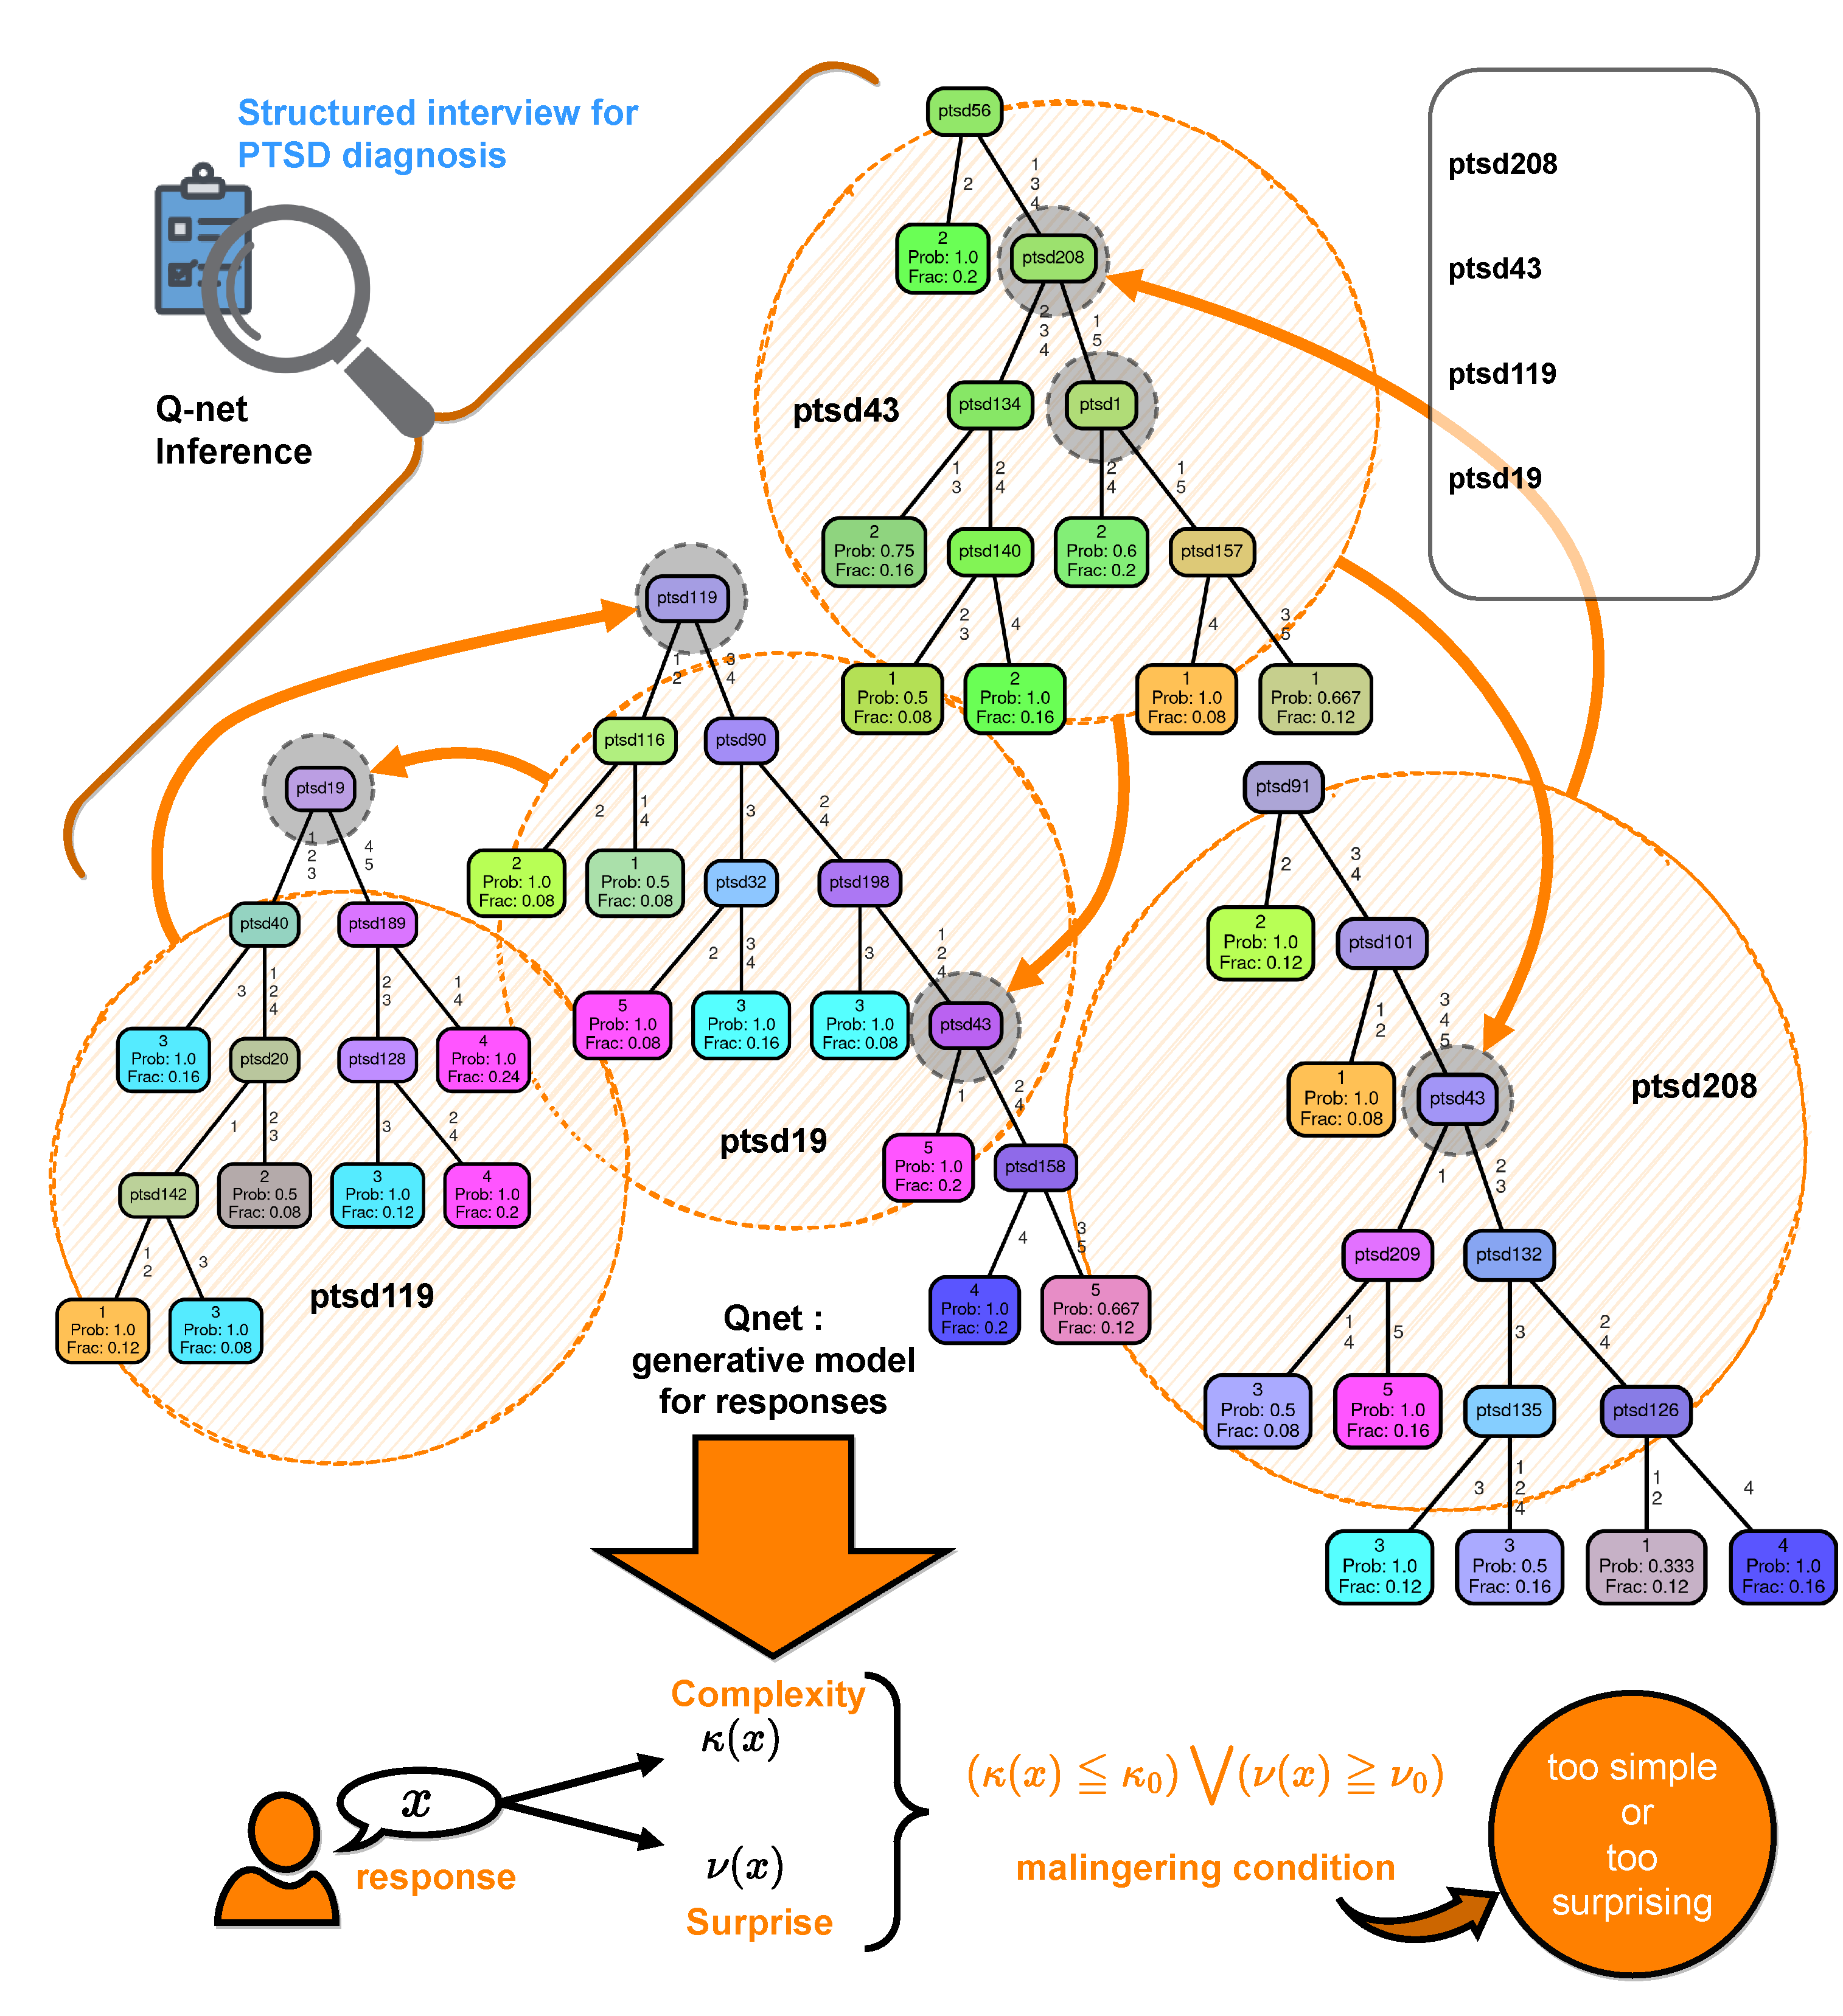
\includegraphics[width=\textwidth]{Figures/qnetptsd}};
    \node [] (B) at ([yshift=1.65in,xshift=-2.35in]A.south) {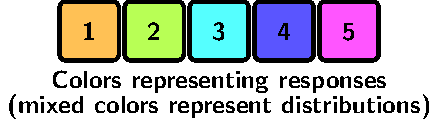
\includegraphics[width=2in]{Figures/test}};
    % \node [text=gray,font=\bf\sffamily\fontsize{8}{8}\selectfont] (C) at ([yshift=7.65in,xshift=-.2in]A.south) {\mnp{6.5in}{\begin{tabular}{C{.25in}L{1.6in}}
  ptsd19 & Feel emotionally numb due to a stressful event in the past?\\
  ptsd43 & Still enjoy doing many things that you used to enjoy? \\
  ptsd119& How often have you experienced memory problems due to a stressful event in the past? \\
\end{tabular}                         }};
                                                                    \end{tikzpicture}
                      
  \else
  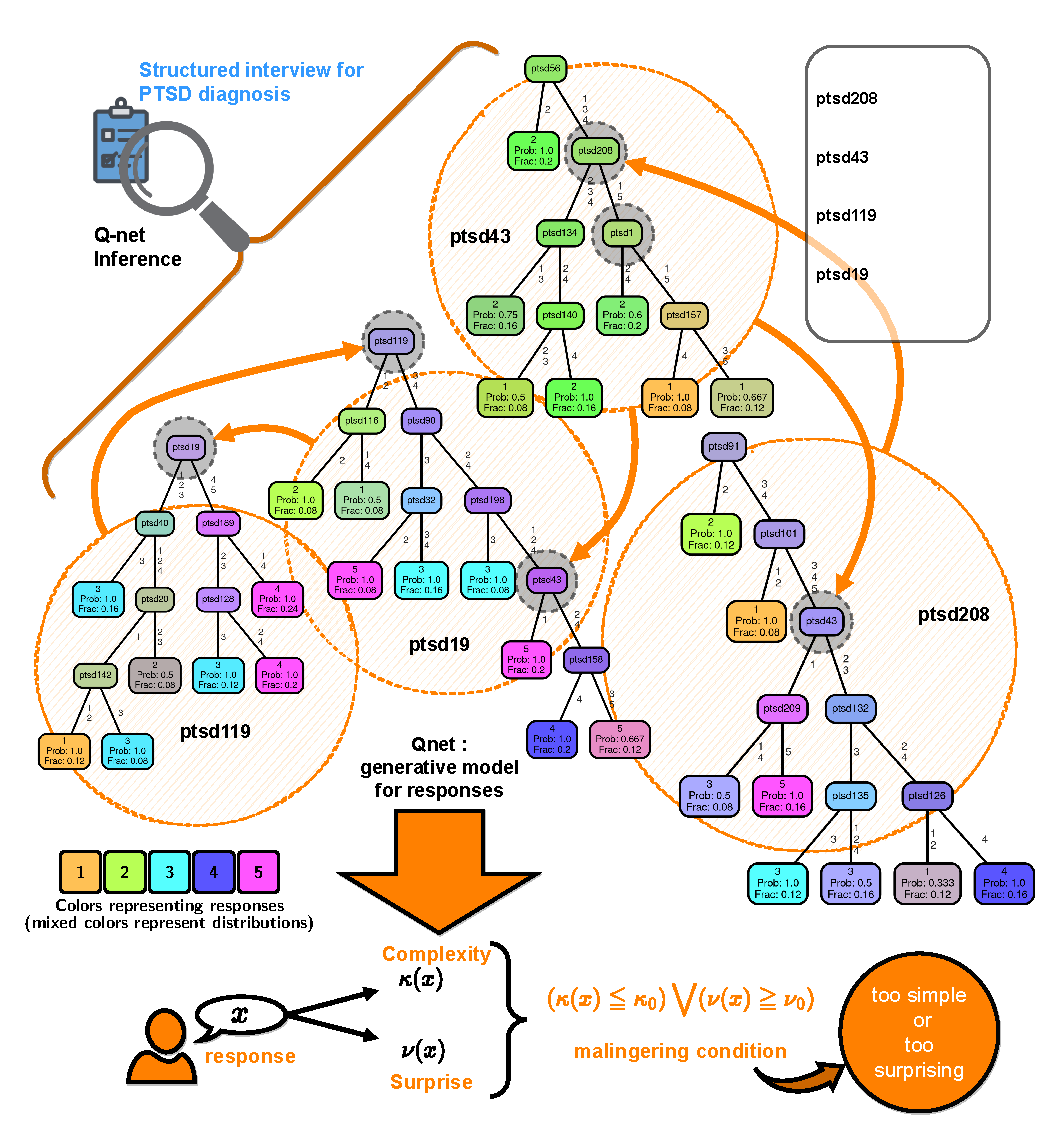
\includegraphics[width=.92\textwidth]{Figures/External/scheme}
  \fi
 
  \vspace{-12pt}
  
  \captionN{\textbf{Conceptual framework.} Using a  dataset of responses to a validated structured interview for PTSD diagnoses, along with physician-validated clinical diagnoses, we infer generative models for responses for PTSD patients. In our framework for detecting  malingering, we flag responses as those which are highly ``surprising'' (defined as violating infered cross-dependencies between  individual response items) or are too simple (lacking complexity in the response patterns typical of non-malingered responses). The precise ``malingering condition'' shown above is validated from theoretical considerations as well as field experimental data.}\label{figscheme}
\end{figure}

\begin{table}[t]
  \centering 
  
  \captionN{Demographic Characteristics and Malingering Success Rates (PL Dataset)$^\star$ at 94.2\% sensitivity}\label{tabprolific}
  \sffamily\fontsize{9}{9}\selectfont
\begin{tabular}{L{1.8in}|L{1.2in}|L{.8in}|L{.8in}|L{1.2in}}\hline
characteristics& mean  Completion  Time  [s] & mean  age  [years] & no.  of  participants & success  rate  (\%) \\\hline
 \rowcolor{\ACOL}Race:  Asian &188.4&34.3&24&8.3\\\hline
 \rowcolor{\ACOL}Race:  Black &329.5&38.0&33&18.2\\\hline
 \rowcolor{\ACOL}Race:  Mixed &195.8&31.4&20&5.0\\\hline
 \rowcolor{\ACOL}Race:  Other &286.2&38.5&13&0.0\\\hline
 \rowcolor{\ACOL}Race:  White &186.5&42.7&220&4.1\\\hline
 \rowcolor{\BCOL}Sex:  Female &201.5&40.5&167&4.8\\\hline
 \rowcolor{\BCOL}Sex:  Male &213.5&41.0&141&7.1\\\hline
 \rowcolor{\CCOL}Residence:  United  Kingdom &213.5&43.1&110&4.5\\\hline
 \rowcolor{\CCOL}Residence:  United  States &202.9&39.4&200&6.5\\\hline
\hline\end{tabular}

\vskip .5em
$^\star$Using $\kappa_0=1,\nu_0=0.76, \mu_0=1.35$.
\end{table}
 
\begin{table}[t]
  \centering
  
  \captionN{Lower Bounds on Performance trade-offs at Different Population Prevalences of PTSD Malingering$^\dag$}\label{tabperf}
  \sffamily\fontsize{9}{11}\selectfont
  
  \begin{tabular}{L{.69in}|L{.75in}|L{.75in}|L{.75in}|L{.75in}|L{.75in}|L{.75in}|L{.75in}}\hline
fpr&tpr&ppv&acc&npv&LR+&LR-&prevalence\\
0.01& $0.893  \pm  0.018$ & $0.900  \pm  0.003$ & $0.979  \pm  0.002$ & $0.988  \pm  0.002$ & $81.27  \pm  2.145$ & $0.107  \pm  0.018$ &0.10\\
0.02& $0.893  \pm  0.018$ & $0.902  \pm  0.003$ & $0.969  \pm  0.003$ & $0.981  \pm  0.003$ & $52.53  \pm  1.680$ & $0.108  \pm  0.018$ &0.15\\
0.02& $0.892  \pm  0.018$ & $0.902  \pm  0.002$ & $0.959  \pm  0.004$ & $0.973  \pm  0.004$ & $37.19  \pm  1.101$ & $0.109  \pm  0.019$ &0.20\\
0.03& $0.892  \pm  0.018$ & $0.902  \pm  0.002$ & $0.949  \pm  0.004$ & $0.964  \pm  0.006$ & $27.88  \pm  0.743$ & $0.111  \pm  0.019$ &0.25\\
\hline\end{tabular}


  \vskip .5em
  
$\dag$ Abbreviations: Population prevalence (prev.), Positive Predictive Value (ppv), Negative Predictive Value (npv), Accuracy (acc), Positive Likelihood Ratio (LR+), Negative Likelihood Ratio (LR-). 99\% confidence  intervals calculated  for $n=310+0.6 \times 304 = 492$.
\end{table}
\begin{table}[t]
  \centering
  
  \sffamily\fontsize{10}{8}\selectfont
 
\captionN{Demographic characteristics of participating mental health professionals}\label{tabpsych}

  

\begin{tabular}{R{3in}L{2in}}
\multicolumn{2}{c}{} \\ 
\rowcolor{lightgray}\textbf{Area of Expertise}   &  \\ 
Neuropsychology             & 11 \\
Forensic Psychiatry         & 8  \\
Psychology                  & 4  \\
Forensic Neuropsychology    & 3  \\
Neurology                   & 1  \\ 
\multicolumn{2}{c}{} \\ % Empty row for spacing
\rowcolor{lightgray}\textbf{Sex}   &  \\ 
Male   & 14 \\
Female & 13 \\ 
\multicolumn{2}{c}{} \\ % Empty row for spacing
\rowcolor{lightgray} \textbf{Primary Institution of Affliation}                          &  \\ 
Northwestern University                      & 21 \\
University of Illinois Chicago               & 3  \\
NorthShore University HealthSystem           & 1  \\
University of Chicago Medicine               & 1  \\
Rush University Medical Center               & 1  \\ 
\end{tabular}



\end{table}


\begin{figure}
  \tikzexternalenable
  \tikzsetnextfilename{perf}
 
  \centering
%\tikzXtrue
  \iftikzX
  \begin{tikzpicture}[font=\bf\sffamily\fontsize{8}{8}\selectfont]

  \begin{groupplot}[
    group style={columns=4,rows=3,horizontal sep=.5in, vertical sep=.6in},
title style={xshift=-.6in,anchor=south east},
    ]
    \def\HGT{1.1in}

    %1
    \nextgroupplot[title={\large (a)},
    axis line style={black, thick},
    width=\HGT, 
    height=\HGT,
    scale only axis=true,
    axis on top=true,
    major tick length=0pt,
    enlargelimits=false,
    % xmin=0,xmax=1,ymin=0,ymax=1,
    grid=both,
    grid style={dashed,semithick,draw=gray, opacity=.25},
    ] % 1
    \pgfplotstableread[col sep=comma]{Figures/plotdata/kappa.csv}\datafileA
    \pgfplotstableread[col sep=comma]{Figures/plotdata/kappa_h.csv}\datafileB
    \addplot[ybar,bar width=1pt,draw=none,fill=Orchid1!80!black,opacity=.5] table[x=x,y=kappa] {\datafileB};
    \addplot[smooth,no marks, ultra thick, black,] table[x=x,y=kappa] {\datafileA};


    
    %2
    \nextgroupplot[title={\large (b)},
    axis line style={black, thick},
    width=\HGT, 
    height=\HGT,
    scale only axis=true,
    axis on top=true,
    major tick length=0pt,
    enlargelimits=false,
    % xmin=0,xmax=1,ymin=0,ymax=1,
    grid=both,
    grid style={dashed,semithick,draw=gray, opacity=.25},
    ] % 1
    \pgfplotstableread[col sep=comma]{Figures/plotdata/nu.csv}\datafileA
    \pgfplotstableread[col sep=comma]{Figures/plotdata/nu_h.csv}\datafileB
    \addplot[ybar,bar width=2pt,draw=none,fill=Orchid1!80!black,opacity=.5] table[x=x,y=mu] {\datafileB};
    \addplot[smooth,no marks, ultra thick, black,] table[x=xd,y=nu] {\datafileA};



    %3
    \nextgroupplot[title={\large (c)},
    axis line style={black, thick},
    axis background/.style={
      shade,top color=transparent!5,bottom color=transparent!1},
    width=\HGT, 
    height=\HGT,
    scale only axis=true,
    enlargelimits=false,
    axis on top=true,
    major tick length=0pt,
    xmin=0,xmax=1,ymin=0,ymax=1,
    grid=both,
    grid style={dashed,semithick,draw=gray, opacity=.25},
    ] % 1
    \pgfplotstableread[col sep=comma]{Figures/plotdata/roc.csv}\datafileA
    \addplot[name path=tprU,smooth,draw=none] table[x=fpr,y=tprU] {\datafileA};
    \addplot[name path=tprL,smooth,draw=none] table[x=fpr,y=tprL] {\datafileA};
    \addplot[Orchid1!80!black,opacity=.5] fill between[of=tprU and tprL];
    \addplot[smooth,no marks, ultra thick, black,] table[x=fpr,y=tpr] {\datafileA};


    %4
    \nextgroupplot[title={\large (d)},
    axis line style={black, thick},
    view={0}{90},
    xtick={0,1,2,3,4},
    xticklabels={$\kappa$,$\nu$,$\mu$,dx,$\chi$},
    ytick={0,1,2,3,4},
    yticklabels={$\kappa$,$\nu$,$\mu$,dx,$\chi$},
    width=\HGT, 
    height=\HGT,
    colormap/pink,
    colorbar horizontal,colorbar style={yshift=0in, height=.1in},
    scale only axis=true,
    axis on top=false,point meta min=-1,point meta max=1,
    major tick length=0pt,
    scale only axis,
    ] % 1
    \addplot3 [raw gnuplot,matrix plot*,mesh/cols=5] gnuplot  {
      plot 'Figures/plotdata/expcorr.csv' matrix with image;
    };

    %5
    \nextgroupplot[title={\large (e)},
    axis line style={black, thick},
    axis background/.style={
      shade,top color=transparent!5,bottom color=transparent!1},
    width=\HGT, 
    height=\HGT,
    scale only axis=true,
    enlargelimits=0.05, 
    axis on top=true,
    major tick length=0pt,
   % colormap/autumn,colorbar horizontal,colorbar style={yshift=0in,at={(0,1.25)},anchor=north west, height=.1in},
    grid=both,
    grid style={dashed,semithick,draw=gray, opacity=.25},
    ] 
    \def\datafileA{Figures/plotdata/vadata_res.csv}
    % \addplot[scatter,only marks,mark=*,mark options={mark size=1.5pt,fill=black,draw=gray,opacity=.5},point meta=explicit,discard if={chi}{-1}] table[col sep=comma,x=kappa,y=nu,meta=mu] {\datafileA};
   % \addplot[scatter,only marks,mark=square*,mark options={mark size=1pt,fill=Red1,draw=gray,opacity=.5},point meta=explicit,discard if not={chi}{-1}] table[col sep=comma,x=kappa,y=nu,meta=nu] {\datafileA};
     \addplot[only marks,mark=*,mark options={mark size=1.25pt,fill=gray,draw=lightgray,opacity=.6},discard if not={DX}{0},discard if={chi}{-1}] table[col sep=comma,x=kappa,y=nu] {\datafileA};
    \addplot[only marks,mark=*,mark options={mark size=1.5pt,draw=Orchid4!50!black,fill=DarkOrange,draw=Orchid1,opacity=.5},discard if not={DX}{1},discard if={chi}{-1}] table[col sep=comma,x=kappa,y=nu] {\datafileA};      \addplot[only marks,mark=square*,mark options={mark size=.9pt,fill=black,draw=black,opacity=1},,discard if not={chi}{-1}] table[col sep=comma,x=kappa,y=nu] {\datafileA};
   % \addplot[only marks,mark=square*,mark options={mark size=1pt,fill=Red1,draw=black,opacity=1},,discard if not={chi}{0}] table[col sep=comma,x=mu,y=nu] {\datafileA};
   % \addplot[only marks,mark=square*,mark options={mark size=1pt,fill=Orchid1,draw=black,opacity=1},,discard if not={chi}{1}] table[col sep=comma,x=mu,y=nu] {\datafileA};


 

    %6
    \nextgroupplot[title={\large (f)},
    axis line style={black, thick},
    axis background/.style={
      shade,top color=transparent!5,bottom color=transparent!1},
    width=\HGT, 
    height=\HGT,
    scale only axis=true,
    enlargelimits=true,
    axis on top=true,
    colormap/viridis,
    major tick length=0pt,
    grid=both,
    grid style={dashed,semithick,draw=gray, opacity=.25},
    ] 
    \def\datafileA{Figures/plotdata/vadata_res.csv}
%      \addplot[scatter,only marks,mark=*,mark options={mark size=1.5pt,fill=black,draw=gray,opacity=.65},point meta=explicit,discard if={chi}{-1}] table[col sep=comma,x=mu,y=nu,meta=DX] {\datafileA};
    % \addplot[scatter,only marks,mark=square*,mark options={mark size=1pt,fill=Red1,draw=gray,opacity=.5},point meta=explicit,discard if not={chi}{-1}] table[col sep=comma,x=mu,y=nu,meta=chi] {\datafileA};
     \addplot[only marks,mark=*,mark options={mark size=1.25pt,fill=gray,draw=lightgray,opacity=.6},discard if not={DX}{0},discard if={chi}{-1}] table[col sep=comma,x=mu,y=kappa] {\datafileA};
    \addplot[only marks,mark=*,mark options={mark size=1.5pt,draw=Orchid4!50!black,fill=DarkOrange1,draw=Orchid1,opacity=.5},discard if not={DX}{1},discard if={chi}{-1}] table[col sep=comma,x=mu,y=kappa] {\datafileA};
\addplot[only marks,mark=square*,mark options={mark size=.9pt,fill=black,draw=black,opacity=1},,discard if not={chi}{-1}] table[col sep=comma,x=mu,y=kappa] {\datafileA};

   

    
    %7
    \nextgroupplot[title={\large (g)},
    axis line style={black, thick},
    width=\HGT, 
    height=\HGT,
    scale only axis=true,
    axis on top=true,
    major tick length=0pt,
    xmin=0,xmax=1,ymin=0,ymax=1,
    grid=both,
    grid style={dashed,semithick,draw=gray, opacity=.25},
    ] % 1
    \pgfplotstableread[col sep=comma]{Figures/plotdata/vroc.csv}\datafileA
    \addplot[smooth,no marks, ultra thick, black,] table[x=fpr,y=tpr] {\datafileA};
    \addplot[name path=tprU,smooth,draw=none] table[x=fpr,y=tprU] {\datafileA};
    \addplot[name path=tprL,smooth,draw=none] table[x=fpr,y=tprL] {\datafileA};
    \addplot[Orchid1!80!black,opacity=.5] fill between[of=tprU and tprL];


    %8
    \nextgroupplot[title={\large (d)},
    axis line style={black, thick},
    view={0}{90},
    xtick={0,1,2,3,4},
    xticklabels={$\kappa$,$\nu$,$\mu$,dx,$\chi$},
    ytick={0,1,2,3,4},
    yticklabels={$\kappa$,$\nu$,$\mu$,dx,$\chi$},
    width=\HGT, 
    height=\HGT,
    colormap/pink,
    colorbar horizontal,colorbar style={yshift=0in, height=.1in},
    scale only axis=true,
    axis on top=false,point meta min=-1,point meta max=1,
    major tick length=0pt,
    scale only axis,
    ] % 1
    \addplot3 [raw gnuplot,matrix plot*,mesh/cols=5] gnuplot  {
      plot 'Figures/plotdata/expcorr.csv' matrix with image;
    };
    
    %9
    \nextgroupplot[title={\large (i)},
    axis line style={black, thick},
    axis background/.style={
      shade,top color=transparent!5,bottom color=transparent!1},
    width=\HGT, 
    height=\HGT,
    scale only axis=true,
    enlargelimits=0.05, 
    axis on top=true,
    major tick length=0pt,
    grid=both,
    grid style={dashed,semithick,draw=gray, opacity=.25},
    ] 
    \def\datafileA{Figures/plotdata/expdata_res.csv}
    \addplot[only marks,mark=*,mark options={mark size=1.25pt,fill=gray,draw=lightgray,opacity=.6},discard if not={DX}{False},discard if={chi}{-1}] table[col sep=comma,x=kappa,y=nu] {\datafileA};
    \addplot[only marks,mark=*,mark options={mark size=1.5pt,draw=Orchid4!50!black,fill=DarkOrange1,draw=Orchid1,opacity=.5},discard if not={DX}{True},discard if={chi}{-1}] table[col sep=comma,x=kappa,y=nu] {\datafileA};    %\addplot[scatter,only marks,mark=*,mark options={mark size=1.5pt,fill=black,draw=gray,opacity=.5},point meta=explicit,discard if={chi}{-1}] table[col sep=comma,x=kappa,y=nu,meta=mu] {\datafileA};
   % \addplot[scatter,only marks,mark=square*,mark options={mark size=1pt,fill=Red1,draw=gray,opacity=.5},point meta=explicit,discard if not={chi}{-1}] table[col sep=comma,x=kappa,y=nu,meta=nu] {\datafileA};
   \addplot[only marks,mark=square*,mark options={mark size=.9pt,fill=black,draw=black,opacity=1},,discard if not={chi}{-1}] table[col sep=comma,x=kappa,y=nu] {\datafileA};
   % \addplot[only marks,mark=square*,mark options={mark size=1pt,fill=Red1,draw=black,opacity=1},,discard if not={chi}{0}] table[col sep=comma,x=mu,y=nu] {\datafileA};
   % \addplot[only marks,mark=square*,mark options={mark size=1pt,fill=Orchid1,draw=black,opacity=1},,discard if not={chi}{1}] table[col sep=comma,x=mu,y=nu] {\datafileA};


 
 

    %10
    \nextgroupplot[title={\large (h)},
    axis line style={black, thick},
    axis background/.style={
      shade,top color=transparent!5,bottom color=transparent!1},
    width=\HGT, 
    height=\HGT,
    scale only axis=true,
    enlargelimits=true,
    axis on top=true,
    colormap/viridis,
    major tick length=0pt,
    grid=both,
    grid style={dashed,semithick,draw=gray, opacity=.25},
    ] 
    \def\datafileA{Figures/plotdata/expdata_res.csv}
%      \addplot[scatter,only marks,mark=*,mark options={mark size=1.5pt,fill=black,draw=gray,opacity=.65},point meta=explicit,discard if={chi}{-1}] table[col sep=comma,x=mu,y=nu,meta=DX] {\datafileA};
    % \addplot[scatter,only marks,mark=square*,mark options={mark size=1pt,fill=Red1,draw=gray,opacity=.5},point meta=explicit,discard if not={chi}{-1}] table[col sep=comma,x=mu,y=nu,meta=chi] {\datafileA};
     \addplot[only marks,mark=*,mark options={mark size=1.25pt,fill=gray,draw=lightgray,opacity=.6},discard if not={DX}{False},discard if={chi}{-1}] table[col sep=comma,x=mu,y=kappa] {\datafileA};
    \addplot[only marks,mark=*,mark options={mark size=1.5pt,draw=Orchid4!50!black,fill=DarkOrange1,draw=Orchid1,opacity=.5},discard if not={DX}{True},discard if={chi}{-1}] table[col sep=comma,x=mu,y=kappa] {\datafileA};
\addplot[only marks,mark=square*,mark options={mark size=.9pt,fill=black,draw=black,opacity=1},,discard if not={chi}{-1}] table[col sep=comma,y=kappa,x=mu] {\datafileA};

   

    %11
    \nextgroupplot[title={\large (g)},
    axis line style={black, thick},
    width=\HGT, 
    height=\HGT,
    scale only axis=true,
    axis on top=true,
    major tick length=0pt,
    xmin=0,xmax=1,ymin=0,ymax=1,
    grid=both,
    grid style={dashed,semithick,draw=gray, opacity=.25},
    ] % 1
    \pgfplotstableread[col sep=comma]{Figures/plotdata/vroc.csv}\datafileA
    \addplot[smooth,no marks, ultra thick, black,] table[x=fpr,y=tpr] {\datafileA};
    \addplot[name path=tprU,smooth,draw=none] table[x=fpr,y=tprU] {\datafileA};
    \addplot[name path=tprL,smooth,draw=none] table[x=fpr,y=tprL] {\datafileA};
    \addplot[Orchid1!80!black,opacity=.5] fill between[of=tprU and tprL];

 
        %12
    \nextgroupplot[title={\large (h)},
    axis line style={black, thick},
    view={0}{90},
    xtick={0,1,2,3,4},
    xticklabels={$\kappa$,$\nu$,$\mu$,dx,$\chi$},
    ytick={0,1,2,3,4},
    yticklabels={$\kappa$,$\nu$,$\mu$,dx,$\chi$},
    width=\HGT, 
    height=\HGT,
    colormap/pink,
    % colorbar horizontal,colorbar style={yshift=.1in, at={(0,1.2)},anchor=north west,height=.1in},
    scale only axis=true,
    axis on top=false,point meta min=-1,point meta max=1,
    major tick length=0pt,
    scale only axis,
    ] % 1
    \addplot3 [raw gnuplot,matrix plot*,mesh/cols=5] gnuplot  {
      plot 'Figures/plotdata/vacorr.csv' matrix with image;
    };

    % \def\datafileA{Figures/plotdata/roc.csv} % Update to the correct file path if needed

  \end{groupplot}
\end{tikzpicture}
  \else
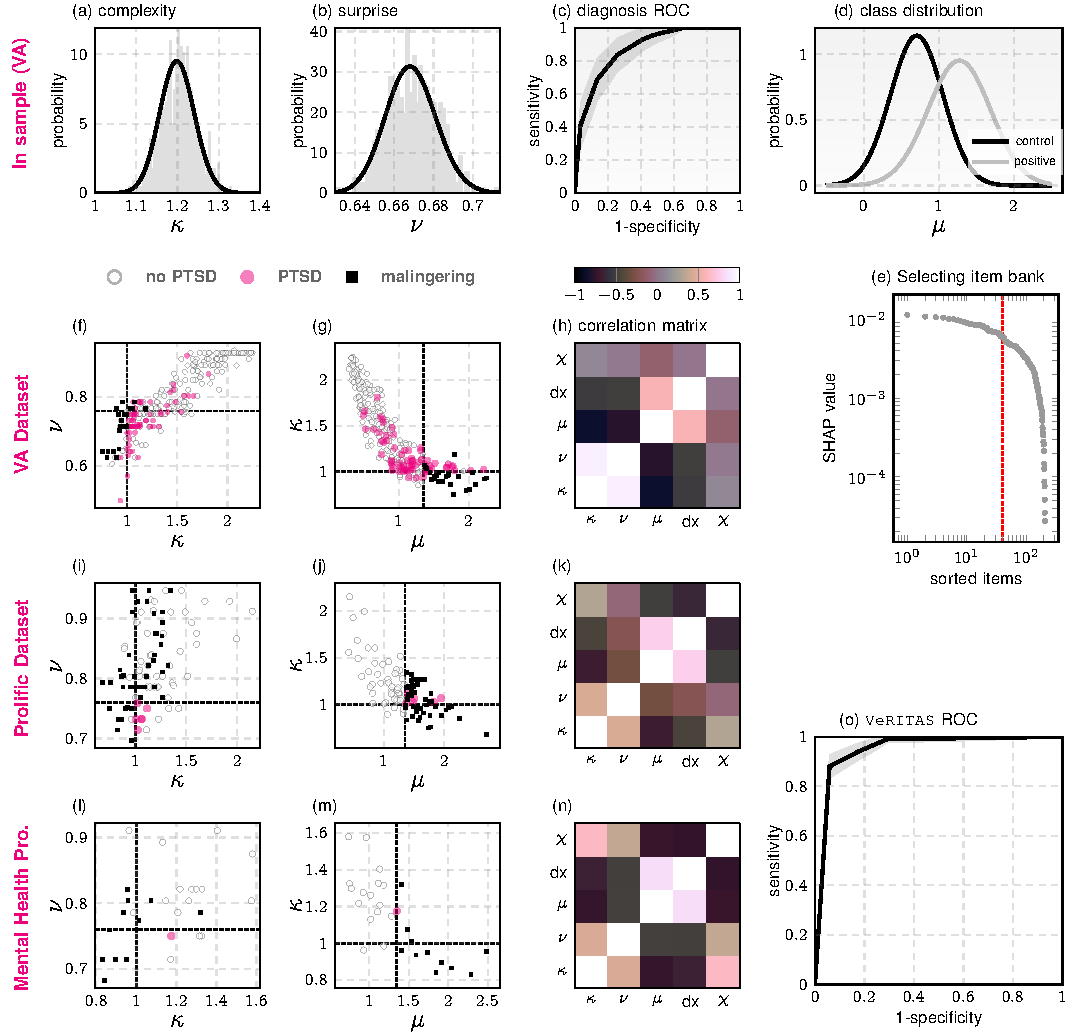
\includegraphics[width=\textwidth]{Figures/External/perf}
  \fi 
  \vspace{-10pt}
  
  \captionN{\textbf{Training and performance.} a, distribution of the complexity parameter. b, distribution of the surprise parameter. c, ROC curve for diagnosis of PTSD without consideration of possible malingering using \qnet models, $i.e.$ using the $\mu$ parameter as risk. d, Class distribution for setting $\mu_0=1.35$. e, distribution of SHAP values of the CAT-PTSD master item bank, showing the threshold above which the \vrts subset is selected. Panels f-n, out-of-sample results for the three datasets, namely out-of-sample portion of the VA dataset, the PL and the PS datasets. Notably, the different categories of responses obtained comprise ones that are deemd to not have PTSD without any need to consider malingering, those which are diagnosed as  having PTSD, and those who are flagged as malingering. Panels h,k,n show  correlation between the three \vrts parameters, and $\chi$ which is an indicator variable for malingering flags. dx is the indiator of physician-confirmed diagnosis (only available for the VA data), or estimated diagnosis using the $\mu_0$ threshold. Panel o illsutrates the lower envelop of teh ROC curve for \vrts, and 95\% confidence bounds.}\label{figperf}
\end{figure}